%!TEX root = Animismus_in_Anime.tex
Bevor im Nachfolgenden die Kriterien zur Feststellung von Animismus in den Anime-Filmen angewendet werden, sollen diese kurz resümiert werden. Es handelt sich dabei um insgesamt zehn Kriterien. Die ersten fünf ergeben sich aus Graham Harveys Untersuchung zum Animismus. Sie sind nummeriert und beginnen mit einem H. Die übrigen fünf Kriterien nach Pascal Boyer sind mit B markiert.
\begin{itemize}
	\item [H1] Animismus ist ein respektvolles Beziehungsgeschehen zwischen Personen, wobei es sich bei Personen auch um Andere-als-Menschen handeln kann.
	\item [H2] Animismus kann sich in der Sprache niederschlagen.
	\item [H3] Animierte Objekte weisen in der Regel anthropomorphe Merkmale auf.
	\item [H4] Das Land ist ein wesentlicher Identifikationsfaktor.
	\item [H5] Durch Veränderung der Umwelt findet eine Transformation statt, die den Veränderer in das Veränderte aufnimmt.
	\item [B1] Anstelle eines Mems konstruiert das menschliche Gehirn anhand einer \emph{Schablone}.
	\item [B2] Die fünf ontologischen Kategorien sind: PERSON, TIER, PFLANZE, NATUROBJEKT, WERKZEUG. Das Verstossen gegen eine dieser ontologischen Kategorien weist auf Übernatürliches hin.
	\item [B3] Übernatürliche Wesen haben Zugang zu sozial-relevanten Informationen. 
	\item [B4] Personen stehen in einer Abhängigkeit zueinander, wodurch sorgfältige Interaktion notwendig wird um Übel abzuwenden.
	\item [B5] Diese Interaktion erfolgt unter anderem anhand von Ritualen, beispielsweise Reinigungsrituale.
\end{itemize} 

\subsection{Mononoke} 
\subsubsection{Konflikt als Resultat fehlenden Respekts} 
Durch seinen historischen Hintergrund fügt sich die Welt des Films von sich aus in den Shinto, und damit in einen geschichtlichen Animismus ein. Die Welt von Mononoke ist voll von verschiedenen \emph{Personen} (H1). Die meisten davon sind Menschen, aber nicht wenige sind Nicht-Menschen-Leute. Es gibt verschiedene Interessensgruppen. Dabei ist es nicht entscheidend, ob es sich um Menschen oder Andere-als-Menschen handelt. Der Konflikt zwischen den Eisenschmiedebewohnern und den Tieren des Waldes ist nicht grösser, als derjenige zwischen den Bewohnern der Eisenschmiede und den Samurai des Königs und sogar die Affengötter werfen mit Steinen nach den Wolfsgöttern. Der respektvolle Umgang zwischen den verschiedenen Menschen und der Andere-als-Menschen-Gruppe steht im Zentrum der Geschichte. Der rücksichtslose Umgang mit den Anderen ist die Ursache der vielen Konflikte. Am Ende ist das Schlimmste zwar abgewendet, aber die Grundproblematik bleibt bestehen und einzig ein gegenseitiger Respekt kann auf den Frieden hoffen lassen. 
 
Die Verbundenheit mit dem Land ist bei San und den Waldgöttern offensichtlich (H4). Doch auch die Bewohner der Eisenschmiede identifizieren sich mit dem Ort an dem sie wohnen. Durch das Abholzen und das Schöpfen von Eisenerz wird die Umwelt stark verändert. Es bedroht die Heimat der Tiere, doch in dieser Veränderung finden die Menschen ihre Lebensgrundlage (H5).

Miyazakis Botschaft in Mononoke ist ein Schuss ins Blaue für den Animismus den Harvey plädiert. Es ist hingegen schwieriger Harveys Beispiele für Animismus in Mononoke anzuwenden. Das Übernatürliche ist so real und fassbar in der Welt von Mononoke, dass es kaum Platz für das stille Belebte lässt, wie zum Beispiel ein geschnitzter Anhänger der Maori oder ein Stein der Ojibwa. Eine Ausnahme bilden allerdings die Kodama. Diese kleinen stummen Geister, die Zeichen für einen gesunden Wald sind, weisen anthropomorphe Züge auf (H3). 

\subsubsection{Die ontologische Kategorie TIER} 
Boyers Ansatz um die Faszination des Übernatürlichen zu erklären, bringt zunächst keine überraschenden Resultate. Vielmehr haben wir mit den Tiergöttern einfache Vorzeigebeispiele des ontologischen Verstosses der Kategorie TIER (B2). Die Tiergötter des Waldes, die Wölfe, die Keiler und auch die Affen handeln, sprechen und denken wie eine PERSON. Angereichert werden sie durch spezielle Merkmale, die aber nur einen Verstoss der Schablone für ihre jeweilige Art darstellt. Die Tiergötter sind alle grösser als ihre natürlichen Verwandten, die Wölfin Moro besitzt zwei Schwänze und der Keiler Okkoto hat eine zusätzliche Reihe von Hauern. Jedoch sind das nicht die ausschlaggebenden Elemente. Das sehen wir am Beispiel von Ashitakas Reittier. Yakul hat ein kräftiges rot-oranges Fell, welches an seiner Unterseite cremig weiss ist. Er weist den Körperbau eines Hirsches auf, ist aber kräftiger und grösser gebaut und er hat zwei lange Hörner anstelle eines Geweihs. Das Tier passt also zu keiner konkreten Vorstellung, die wir haben, aber es passt zu jener Schablone (B1), die Rehe, Gämsen und Elche mit einschliesst. Damit ist es auffällig, reiht sich aber nicht in die Vorstellungen religiöser Phänomene ein. 

Bei genauer Betrachtung kann man der Wolfsgöttin Moro bzw. dem Mädchen San einen weiteren Bruch zuschreiben, da die beiden in einer Mutter-Tochter Beziehung stehen (H1), und weil das über die ontologische Kategorie von TIER bzw. PERSON hinaus geht (B2). Da es sich aber explizit um eine Adoption handelt, sollte dieser Punkt nicht für sich alleine stehen und in das PERSON-Sein von Moro eingeschlossen werden. 

Interessanter und zugleich schwieriger für die Untersuchung mit Boyers Methoden ist der Waldgott Shishigami. Es ist nicht einfach, diesen Waldgott einzuordnen. Während des Tages streift er mit einer Herde Rehe durch den Wald. Bei Nacht wechselt er die Form und kann ohne Widerstand durch den Wald hindurch laufen. Er ähnelt einem Hirsch, hat aber ein menschliches Gesicht (H3). Er spricht nicht, kann aber mit seiner Berührung Leben nehmen oder geben (B4). Er läuft im Wald und ist zugleich der Geist des Waldes. Shishigami scheint voller Brüche und Verstösse in unseren Schablonen und Kategorien. Er bricht so viele Annahmen, dass es schwer ist ihn überhaupt einer ontologischen Kategorie zu zu ordnen. Wichtiger ist, dass der Shishigami Dinge \emph{weiss}. Als Rezipient und wohl auch als Charakter im Film fragt man sich, wie der Waldgott entscheidet, wen er tötet und wen er heilt. Es könnte pure Willkür sein, doch der Gedanke liegt näher, dass der Waldgott über schicksalhafte \emph{Informationen} (B3) verfügt. Wie Boyer es beschreibt, zeigt sich denn auch, dass dieses Wissen eine wichtige Rolle im sozialen Umfeld spielt. Als der Keilergott halb wahnsinnig zum Waldgott stürmt, geht er davon aus, dass Shishigami \emph{weiss}, dass er und seine Krieger tapfer gekämpft haben und den Wald verteidigen. 

Im Ritual (B5), das die Seherin, aus dem Dorf, aus dem Ashitaka stammt, ausführt, soll der böse Geist des gefallenen Dämon besänftigt und dadurch das Dorf geschützt werden (B4). Somit entspricht dieses Ritual Boyers Beschreibung von religiösen Ritualen. Denn darin geht es im Wesentlichen darum, sich präventiv vor etwas zu schützen. Um den unheimlichen Eindruck zu verstärken, den man sowieso schon vor Leichen hat, kommt hier hinzu, dass der Dämon, obwohl er schon gestorben ist, noch einen Fluch für alle hörbar spricht.\footnote{Vergleiche letzter Abschnitt in Kapitel 1.4, \emph{Beschaffenheit des Übernatürlichen.}}

Um sich mit der Frage zu beschäftigen, ob und welche Rolle der Animismus in der Sprache (H2) spielt, in welcher der Film handelt, wäre es notwendig sich ausführlich mit der japanischen Sprache zu beschäftigen. Damit liesse sich sicherlich Interessantes aus den verwendeten Namen und deren Verwendung herauslesen. Das ist jedoch im Rahmen dieser Arbeit nicht möglich. 

\subsection{Wandelndes Schloss} 
\subsubsection{Alles lebt} 
Abgesehen von der Magie gleicht die Welt, in der die Geschichte spielt, der Unseren. Und vor nicht all zu langer Zeit, einer Zeit, in der man anderen Kulturen nach gesagt hat, dass sie \emph{primitiv} seien, weil sie an eine beseelte Welt glauben. Natürlich lässt sich unsere Vergangenheit nicht mit der Märchenwelt aus dem Film gleichsetzen. Es soll aber vor Augen geführt werden, dass der hier anzutreffende Animismus ein anderer als jener von Mononoke ist. 

Der Feuerdämon ist mehr als nur beseelt, er ist durch das Herz in Lebendiges verwandelt worden (Vgl. Der Begriffe \emph{animare} (lat) bedeutet beleben, beseelen, Lebendiges verwandeln). Calcifer redet und interagiert mit den übrigen Bewohnern des Schlosses. Das macht ihn, wenn man Harveys Ansatz folgt, eindeutig zu einer Person. Um es für den Betrachter einfacher zu machen, das Feuer als Person zu sehen, bekommt Calcifer zwei grosse Glupschaugen und einen Mund von variabler Grösse, in den er sich gerne Holzstücke rein stopft (H3). Die Augen sind in der Regel rund, weisse Kreise mit schwarzen Pupillen. Mit dem Flackern seines ganzen Körpers verändert sich die Form der Augen zwischendurch unmerklich, so dass sie schlitzförmiger werden und einen gefährlichen (dämonischen) Eindruck machen. Seine Flammenform, welche keine feste Umrisslinie hat, flackert beständig und von Zeit zu Zeit lösen sich kleine Flämmchen von ihm. Calcifer gehört also sicherlich zu jenen Anders-als-Menschen, mit denen man schon alleine der Vorsicht wegen mit Respekt begegnen sollte. Obwohl das Feuer freundlich sein kann, schimmert immer wieder seine dämonische und unberechenbare Seite hindurch. 

Der Name Calcifer, zusammengesetzt aus dem lateinischen Genitiv zu \emph{Calx} und dem Verb \emph{ferre}, bedeutet soviel wie Kalkträger (H2). Kalk ist ein seit dem alten Rom wichtiges Material, das beim Bau von Häusern verwendet wird. Im übertragenen Sinn ist Calcifer \emph{der, der das Haus herumträgt}.

Aus Sicht von Harvey macht es wenig Sinn zwischen dem Feuer Calcifer und dem wandelnden Schloss zu unterscheiden, da beides ineinander über geht. Nichtsdestotrotz verfügen beide Aspekte, Calcifer und das Schloss, über ein eigenes, menschenähnliches Gesicht (H3).\todo{Bildli}

%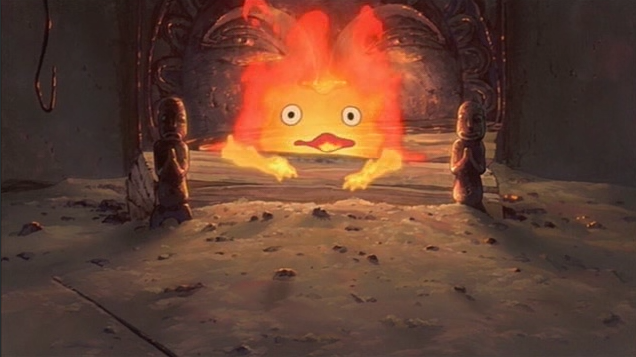
\includegraphics[scale=0.4]{images/00-21-29_calcifer.png}

Sophie zeigt allen gegenüber einen respektvollen und hilfsbereiten Umgang (H1). Sei dies nun Hauro, Markl (Hauros junger Assistent) oder die Hexe aus dem Ödland, seien dies die Menschen oder der Rübenkopf und Calcifer als Andere-als-Menschen. Was einem nur klar wird, wenn man auch die Buchvorlage von Jones gelesen hat, ist, dass Sophie selbst eine magische Fähigkeit besitzt Dinge zu \emph{beleben} (H5). Es ist daher nicht verwunderlich, dass Sophie vorsichtshalber mit allem einen anständigen Umgang pflegt.

Eine Identifikation mit dem Land finden wir in dieser Geschichte nicht. Durch das wandelnde Schloss lebt Hauro und seine Gefährten überall und sind nirgendwo zu Hause. Besonders deutlich wird das durch die magische Eigenschaft des Schlosses, seine Türe an verschiedenen Orten öffnen zu können (H4).

\subsubsection{Das Haus, ein WERKZEUG} 
Ist ein Haus ein Werkzeug (B2)? Im ersten Moment scheint die Idee etwas abwegig, doch das liegt wohl daran, dass das gleiche System, welches Boyer beschreibt, bei der Reflexion des Wortes Werkzeug die Schablone \emph{Handwerkzeuge} gebraucht. Ein Schraubenzieher, ein Hammer, vielleicht auch ein Handmixer - das alles passt zur Schablone (B1) der Handwerkzeuge. Mit Hilfe des Ausschlussverfahrens kommt man jedoch zum Schluss, dass auch ein Haus ein Werkzeug ist. Schliesslich ist ein Werkzeug etwas (in der Regel) Menschengemachtes, das eine Funktion oder einen Zweck erfüllen soll. Mit dieser Beschreibung können wir also getrost sagen, dass ein Haus zur ontologischen Kategorie WERKZEUG gehört. Für das wandelnde Schloss erwarten wir nach Boyer jetzt einen Bruch, der diese Kategorie verletzt. Eine weitere Eigenschaft von Werkzeugen besteht darin, dass sie (so fern sie funktionieren) die Absicht eines Menschen erfüllen. Werkzeuge haben keine Selbstbestimmung. Und genau darüber verfügt das wandelnde Schloss. Es lässt sich argumentieren, dass das Schloss vom Feuerdämon Calcifer belebt und gesteuert wird. Die Verletzung der ontologischen Kategorie bleibt jedoch die gleiche, mit dem Unterschied, dass es statt dem WERKZEUG, zu dem das Haus gehört, nun ein NATUROBJEKT ist. In beiden Fällen wird der Eindruck dadurch verstärkt, dass Eigenschaften einer anderen ontologischen Kategorie in das Aussehen einfliessen. 

Calcifer und Hauro haben zusammen einen Pakt geschlossen. Sie sind von einander abhängig, passiert dem Einen etwas, so besteht auch Gefahr für den Anderen (B4). Dies äussert sich zum Beispiel in Calcifers Sorge um Hauro, als dieser so viel Magie anwendet, dass er droht davon verschlungen zu werden. Und umgekehrt, als Sophie in ihrem Putzwahn vergisst Holz nach zu legen und somit beinahe das Feuer ausgehen lässt. Als sie später in der Geschichte Wasser über Calcifer wirft, als dieser droht die Hexe aus dem Ödland in seinen Flammen zu verzehren, glaube Sophie beide umgebracht zu haben.

An einer Stelle in der Geschichte entscheidet sich Hauro, das wandelnde Schloss neu zu modelieren, insbesondere für Sophie, damit auch sie einen Raum hat und sich wohl fühlt. Um das zu erreichen sind wichtige Vorbereitungen zu treffen: Draussen muss auf dem Boden mit Pulverkreide eine symbolische Markierung gezeichnet werden, in welche sich das wandelnde Schloss begeben muss. Im Schloss innen zeichnet Hauro einen ähnlichen Kreis mit Kreide auf den Boden. Zusammen mit Calcifer schreitet er in diesen Kreis hinein um mit der Verwandlung zu beginnen. Dass dieses Ritual notwendig ist und dafür dient, dass kein Übel passiert, sehen wir in der Szene, wo Calcifer von Sophie aus dem Schloss getragen wird und alles unkontrolliert einstürzt (B5).

Personen, insbesondere solche mit übernatürlichen Kräften, verfügen in dieser Geschichte über Informationen (B2), bei denen es nicht klar ist, woher diese stammen.\begin{quote} \glqq That's some spell you're under. It won't be easy to break.\grqq \end{quote} Ist das erste, was Calcifer zu Sophie sagt, als sie das erste Mal das Schloss betritt. Doch auch schon vorher wird Sophie unfreiwillig als Bote der Hexe aus dem Ödland benutzt um Hauro eine Nachricht zu bringen. 